\documentclass[presentation.tex]{subfiles}

\begin{document}

\begin{frame}
  \frametitle{Ordinary Least Squares (OLS) Regression - Quick Recap}
  \begin{itemize}
    \item A crucial component of BFAST
    \item Linear Model
      \[
      \mathrm{Y} = \mathrm{X}\beta + \varepsilon
      \]
    \item Wish to find a solution to a quadratic minimization problem
      \[
      \hat{\beta} = \operatorname{argmin}_{\beta} \|Y-\mathrm{X} \boldsymbol{\beta}\|^{2}
      \]
    \item $\hat{\beta}$ is the OLS estimator for $\beta$ and can be found using the explicit formula:
      \[
      \hat{\boldsymbol{\beta}}=\left(\mathrm{X}^{\top} \mathrm{X}\right)^{-1}\mathrm{X}^{\top} \mathrm{Y}
      \]
    \item A numerically stable solution can be obtained using QR-decomposition or Moore-Penrose
      pseudoinverse of $\mathrm{X}$ (an expansive topic in itself).
  \end{itemize}
\end{frame}

\begin{frame}
\frametitle{OLS-Regression for Non-linear Functions}
\begin{itemize}
\item Linear regression can be used to estimate linear parameters for
  non-linear functions.
\item E.g. $f(x) = 25 + 2x^{1.2} + 3 \sin{x}$, then:
  \[
  \mathrm{X} = 
  \begin{bmatrix}
    1 & x_1^{1.2} & \sin{x_1}\\
    1 & x_2^{1.2} & \sin{x_2}\\
    \vdots & \vdots & \vdots \\
    1 & x_n^{1.2} & \sin{x_n}
  \end{bmatrix}
  \quad
  \beta =
  \begin{bmatrix}
    25 \\
    2 \\
    3
  \end{bmatrix}
  \]
\end{itemize}
\end{frame}


\begin{frame}
  \frametitle{OLS Example}
  \begin{figure}[H]
    \centering
    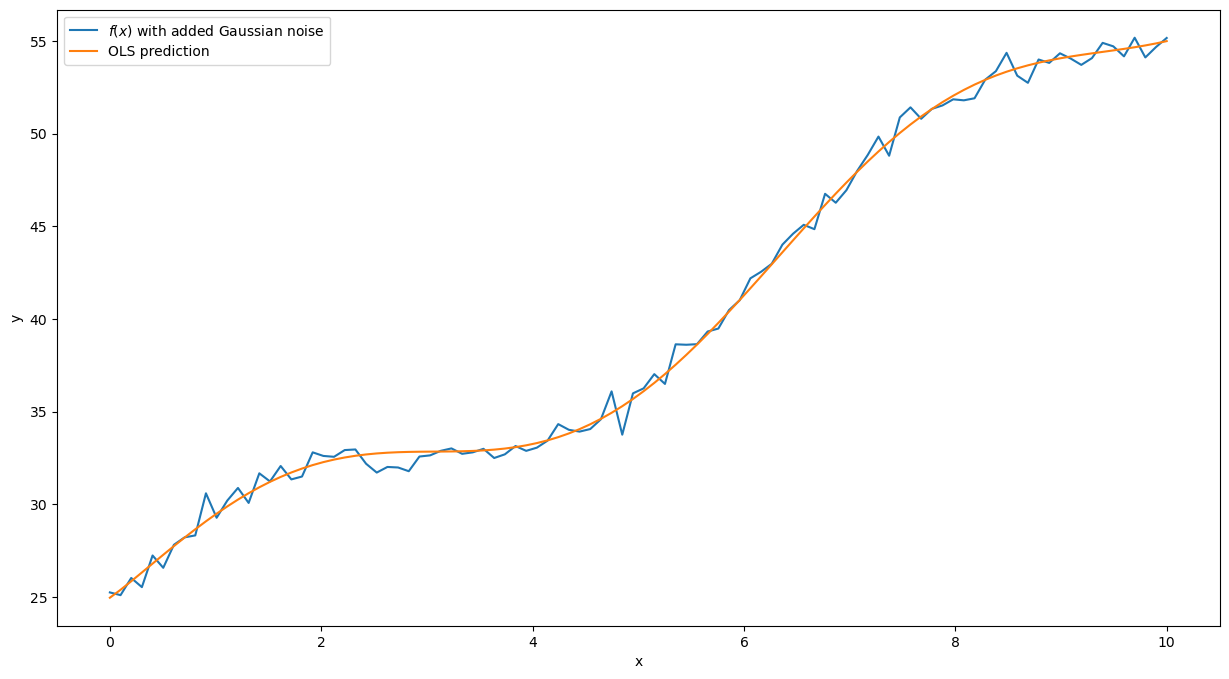
\includegraphics[width=0.8\textwidth]{imgs/ols1.png}
  \end{figure}
\end{frame}
\end{document}
